%\VignetteDepends{MAMA,methods, metaArray,  xtable, metaMA, gtools, gplots, multtest, RankProd, MergeMaid, GeneMeta} 
% \VignetteIndexEntry{An R Package for Meta-Analysis of Microarray}
% \VignetteKeywords{Microarray}
% \VignettePackage{MAMA}

\documentclass[a4paper]{report}
\usepackage{url}
\title{MAMA: an R package for Meta-Analysis of MicroArray}
\author{Ivana Ihnatova}

\usepackage{Sweave}
\begin{document}

\maketitle
\tableofcontents
\newpage
\chapter{Introduction}
%It is well-known that analysis of microarray is statistically difficult and results differ even in repeated experiments.  \par

%By combining data sets from different origins together, the test gets increased power, which leads to more identified genes \cite{Hong}.


%There are three main objectives in analysis of microarray: class comparison (finding of differentially expressed genes), class prediction (prognostic prediction) and class discovery (clustering or unsupervised analyses). 
This paper provides a user guide to the R-package MAMA. The package implements eight different methods that are designed to identify differentially expressed genes in meta-analysis of microarrays. A more comprehensive vignette can be downloaded from: \url{http://is.muni.cz/www/184415/MAMA_full.pdf} \par
                                                                              
In here, we will demonstrate the features of the package with an example of meta-analysis in cancer microarray data, the comparison of expression profiles in MSI (microsatelite instable) and MSS (microsatelite stable) colon cancer. We gathered three microarray data from public databases. The data are stored in {\ttfamily ColonData}. It is an object of new S4 class - {\ttfamily MetaArray}, in which separate slots for gene expression data matrices (expression profiles), clinical sample characteristics and datanames were defined. \par
We start with package and sample data loading. 
\begin{Schunk}
\begin{Sinput}
> rm(list=ls(all=TRUE))
> options(width=60)
> library(MAMA)
> data(ColonData)
> ColonData
\end{Sinput}
\begin{Soutput}
Dataset Denmark  containing 500 probes and  77 samples. 
Sumarization of samples: 
MSIstatus 
--------- 
MSI MSS 
 39  38 
age 
--- 
   Min. 1st Qu.  Median    Mean 3rd Qu.    Max. 
  36.00   45.00   54.00   54.92   62.00   80.00 

Dataset Australia  containing 500 probes and  36 samples. 
Sumarization of samples: 
MSIstatus 
--------- 
MSI MSS 
  5  31 
age 
--- 
   Min. 1st Qu.  Median    Mean 3rd Qu.    Max. 
  50.00   57.75   66.00   66.36   73.75   85.00 

Dataset Japan  containing 500 probes and  41 samples. 
Sumarization of samples: 
location 
-------- 
  distal proximal  unknown 
      28       11        2 
MSIstatus 
--------- 
MSI MSS 
 16  25 
age 
--- 
   Min. 1st Qu.  Median    Mean 3rd Qu.    Max. 
  40.00   47.00   53.00   53.61   60.00   65.00 
\end{Soutput}
\end{Schunk}
The original data sets have been preprocessed and subsampled in order to reduce the computational complexity of the meta-analysis. All data sets have been normalized and are in $log_2$-scale. The corresponding sample sizes for the three datasets can be seen in outprint above. The same set of 500 gene has been selected in each dataset.\par 
A different method is described in each of the parts below and the descriptions are independed from each other, so you can directly move to the method of your interest. %Meta-analysis usually consist of three steps: Data preparation, Detection of differentially expressed genes and Extraction and visualization of results. 
A wrapper function for each method outperforms all necessary steps as one-line command.\par
We select the genes at significance level of 0.05 in all methods. 
 
\chapter{Methods that combine p-values}
%\addcontentsline{toc}{chapter}{Methods that combine p-values}
\section*{Introduction}
%\addcontentsline{toc}{section}{Introduction}
In this part we will focus on methods that combine p-values \cite{Marot}, \cite{Rhodes}. These methods are inspired by Fisher's S-statistic published in 1925 \cite{Fisher25}. \par
Two measurements of significance of change in gene expression are the most common. These are: value of test-statistic and p-value. In here, the p-values from study-specific analysis are combined into one p-value in sense of sum of logs. Methods differ in test statistic used to calculate the study-specific p-values. 
\section*{Usage}
%\addcontentsline{toc}{section}{Usage}
Function {\ttfamily metaMA} is a wrapper funcion for this method. By
\begin{Schunk}
\begin{Sinput}
> pval<- metaMA(ColonData, "MSIstatus", which ="pval")
\end{Sinput}
\begin{Soutput}
    DE    IDD   Loss    IDR    IRR 
212.00  43.00  22.00  20.28  11.52 
\end{Soutput}
\end{Schunk}
we combine study specific p-values({\ttfamily pval}) in {\ttfamily ColonData} dataset using column {\ttfamily "MSIstatus"} from clinical data as class labels. {\ttfamily pval} is a list with seven slots.   \emph{Study1} to \emph{Study3} are numeric vectors with indices of differentially expressed genes in data sets 1 to 3. \emph{AllIndStudies} is a vector of indices of differentially expressed genes in at least one data set. Differentially expressed genes found by meta-analysis have their indices stored in \emph{Meta}. A slot called \emph{TestStatistic} is a vector with test statistics in meta-analysis. The last slot \emph{gene.names} contains the names of the genes in the analysis.  


\chapter{Methods that combine effect sizes}
%\addcontentsline{toc}{part}{Methods that combine effect size}
\section*{Introduction}
%In the situation where $k$ microarray data sets are available and we want to estimate the mean difference in expression, for each gene, between two classes (e.g MSI and MSS colon cancer).\par
Methods that combine effect size use hierarchical model:
\[ y_i=\theta_i+\epsilon_i, \epsilon_i \sim N(0,\sigma_i^2)\]
\[ \theta_i=\mu+\delta_i, \delta_i \sim N(0,\tau_i^2),\]
where $\mu$ is true difference in mean expression between two classes, $y_i$ denotes the measure effect for study $i$, with $i=1,..,k$, $\tau^2$ represents the between study variability, $\sigma_i^2$ denotes the within study variability. The analysis is different depending on whether a fixed-effect model (FEM) or a random-effect model (REM) is deemed appropriate. Under a FEM, $\tau=0$ is assumed, otherwise a REM need to be fit. The estimates of the overall effect $\mu$ are different depending on which model is used. \par
Two papers dealing with effect size combination as method for meta analysis of microarray have been published \cite{Marot} and \cite{Choi2003}. They differ in effect size definition and implementation.\par 
Method presented in \cite{Marot} offers three variants of effect sizes (classical and moderated T-test) and uses explicitly random-effect model. It is implemented as two functions {\ttfamily EScombination} for unpaired data and {\ttfamily EScombination.paired} for paired data.  
\par On the other hand, in \cite{Choi2003} the effect size is defined as Hedge's and Olkin's $g$ and both random-effect and fixed-effect are available. Package \emph{GeneMeta} \cite{GeneMeta} implements this method. 
\section*{Algorithm}
\begin{enumerate}
\item Data recoding.
\item Effect size calculation in each data set.
\item Decision between random-effect model (REM) and fixed-effect model (FEM).
\item Model application.
\item Identification of differentialy expressed genes.
\end{enumerate}
%\addcontentsline{toc}{section}{Introduction}
\section*{Usage}
Because there are two different ways of implementation of this method, we will discuss them separately.
%\addcontentsline{toc}{section}{Usage}
\subsection*{Implementation from metaMA package}
\begin{Schunk}
\begin{Sinput}
> es <- metaMA(ColonData, "MSIstatus", which = "ES")
\end{Sinput}
\begin{Soutput}
    DE    IDD   Loss    IDR    IRR 
166.00  27.00  52.00  16.27  27.23 
\end{Soutput}
\end{Schunk}
This object is a list with seven slots. \emph{Study1} to \emph{Study3} are indices of differentially expressed genes in data sets 1 to 3. \emph{AllIndStudies} is a vector of indices of differentially expressed genes in at least one data set. Differentially expressed genes found by meta-analysis have their indices stored in \emph{Meta}. A slot called \emph{TestStatistic} is a vector with test statistics ("combined effect size") in meta-analysis. The last slot \emph{gene.names} contains the names of the genes in the analysis (rownames of the gene expression data matrices). 
\subsection*{Implemenetation from GeneMeta package}
Function ({\ttfamily ES.GeneMeta}) wrapes data preparation and functions {\ttfamily zScore}, {\ttfamily ScoresFDR}.
\begin{Schunk}
\begin{Sinput}
> es2<-ES.GeneMeta(ColonData, "MSIstatus", nperm = 100)
\end{Sinput}
\end{Schunk}
{\ttfamily nperm = 100} is used only for computational complexity. A thousand of permutation is more appropriate.  
We get a list with two slots. Columns of the first one ({\ttfamily theScores}) refer to:
\begin{itemize}
\item \emph{Effect\_Ex\_ } are the unbiased estimates of the effect 
\item \emph{EffectVar\_Ex\_ } are the estimated variances of the unbiased effects 
\item \emph{zSco\_Ex\_} are the unbiased estimates of the effects divided by their standard deviation 
\item \emph{Qvals} are the Q statistics and \emph{df} is the number of combined experiments minus one
\item \emph{MUvals} and \emph{MUsds} are the overall mean effect sizes and their standard deviations 
\item \emph{zSco} are the z scores  
\item \emph{Qpvalues} is for each gene the probability that a chi-square distribution with \emph{df} degree of freedom has a higher value than its $Q$ statistic
\item \emph{Chisq} is the probability that a chi-square distribution with 1 degree of freedom has a higher value than \emph{zSco2}
\end{itemize}

and the second one (\emph{ScoresFDR}) is a list with three slots: {\ttfamily pos}, {\ttfamily neg} and {\ttfamily two.sided}. The first slot stores the results of the calculation, if the FDR is computed for the positive Z-scores, the second for the negative Z-scores and the last one for the two sided situation. Each slots contains a matrix with similar structure as {\ttfamily theScores} with additional FDR for each data set and combination.\par  


\chapter{Similarity of Ordered Gene Lists (SOGL)}
%\addcontentsline{toc}{part}{Similarity of Ordered Gene Lists (SOGL)}
\section*{Introduction}
%\addcontentsline{toc}{section}{Introduction}
Similarity of Ordered Gene Lists is another method for meta-analysis of microarray. It is call as "comparison of comparisons" by its authors \cite{SOGL}. \par
Briefly, it assigns a similarity score to a comparison of ranked (ordered) gene lists. The score is based on the number of overlapping genes in the top ranks. It computes the size of overlap for each rank. The final score is a weighted sum of these values, with more weight put on the top ranks. \par
\section*{Algorithm}
\begin{enumerate}
\item Required data sets - data sets with same set of genes are required. 
\item Ranking of genes - The genes are then ranked based on gene-wise test on difference of class mean. There is only one assumption about test result: a large positive test score corresponds to up-regulation and a large negative value to down-regulation. 
\item Computing the overlap - for each rank (from 1 to number of genes) we count the number of genes that appear in both ordered lists up to that position. It is denoted as $O_n(G_A,G_B)$, where $G_A$ and $G_B$ refer to ordered gene lists.
\item Similarity score - First we compute a total overlap $A_n$ at position $n$ given as $O_n(G_A,G_B)+O_n(f(G_A),f(G_B))$, where $f()$ means flipped list (down-regulated genes on top). Later we add weights to it and we sum it up to preliminary score. Weights $w_\alpha=e^{-\alpha.n}$ are used as default and tunning of parameter $\alpha$ is needed. The weights are used to put more importance on top genes. 

\end{enumerate}
The algorithm above is valid for meta-analysis in which expression data are not available. However, in this situation we can not use same approach for tunning $\alpha$. 
\section*{Usage}
%\addcontentsline{toc}{section}{Usage}

Function {\ttfamily performSOGL} calculates the similarity score, its statistical significance and the genes responsible for the score.
\begin{Schunk}
\begin{Sinput}
> SOGL.res <- performSOGL(ColonData, varname = "MSIstatus", 
+ test = "FCH", B = 100, which=c("score", "empirical"), 
+ min.weight = 1e-05, two.sided = TRUE )
\end{Sinput}
\begin{Soutput}
Processing data...Tuning alpha..Significance and genes...
\end{Soutput}
\end{Schunk}
{\ttfamily SOGL.res} is a list that contains:
\begin{itemize}
\item \emph{ordering} ordered gene lists as a data.frame where columns refer to datasets
\item \emph{alpha.selected} selected value of alpha parameter 
\item \emph{alpha.considered} vector of alpha considered for selection
\item \emph{pAUC} pAUC values related to all alphas considered
\item \emph{random} random scores (permutations of class labels)
\item \emph{subsample} scores after subsampling from each class and dataset
\item \emph{emp.ci} empirical confidence intervals for number of overlapping genes
\item \emph{common.genes} vector of number of overlapping genes
\item \emph{score} observed similarity score
\item \emph{significance} significance of the observed score in form of p-value
\item \emph{genes} genes that account for observed similarity score
\end{itemize}

The {\ttfamily SOGL.res} is an object of class {\ttfamily SOGLresult} for which plot function exist. 
\begin{Schunk}
\begin{Sinput}
> plot(SOGL.res, "alpha selection") 
\end{Sinput}
\end{Schunk}
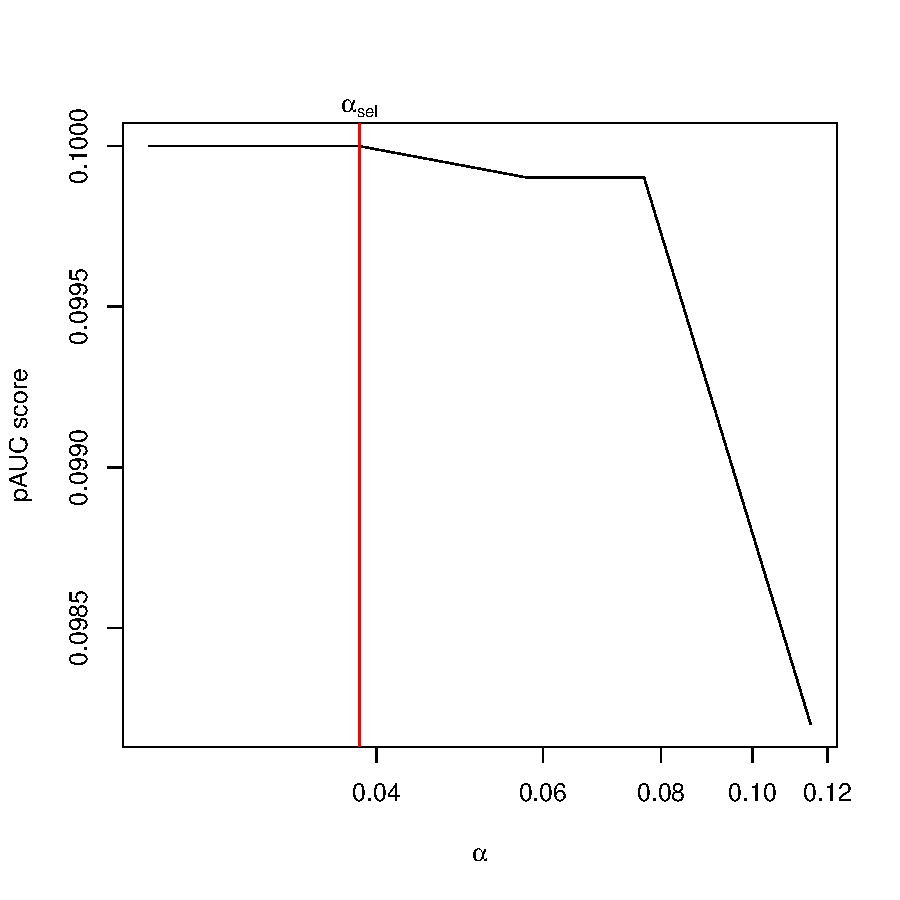
\includegraphics{MAMA-006}

The graph shows pAUC of all $\alpha$'s considered. The selected $\alpha$ is singed by red vertical line. \par
\begin{Schunk}
\begin{Sinput}
> plot(SOGL.res, "density") 
\end{Sinput}
\end{Schunk}
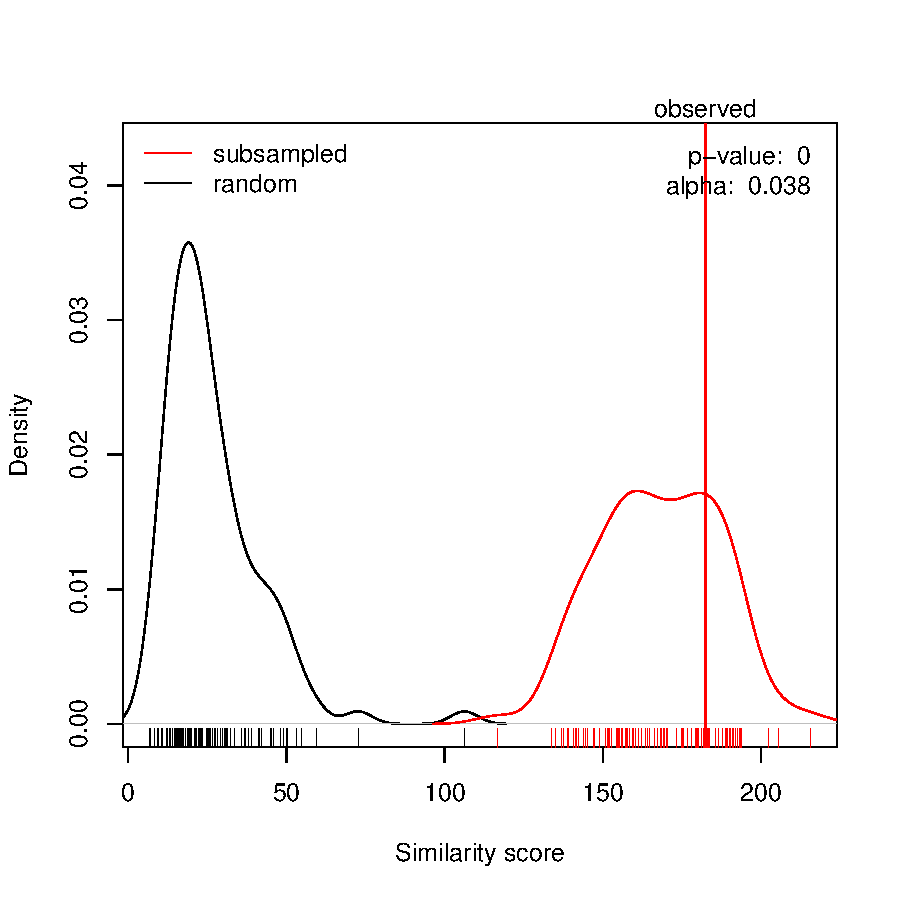
\includegraphics{MAMA-007}

This plots the estimated densities of random (in black) and subsampled score (in red) for selected $\alpha$. The observed similarity score is marked by vertical line. The bottom rugs are scores actually achieved in permutations. 
\begin{Schunk}
\begin{Sinput}
> plot(SOGL.res, "empirical CI")
\end{Sinput}
\end{Schunk}
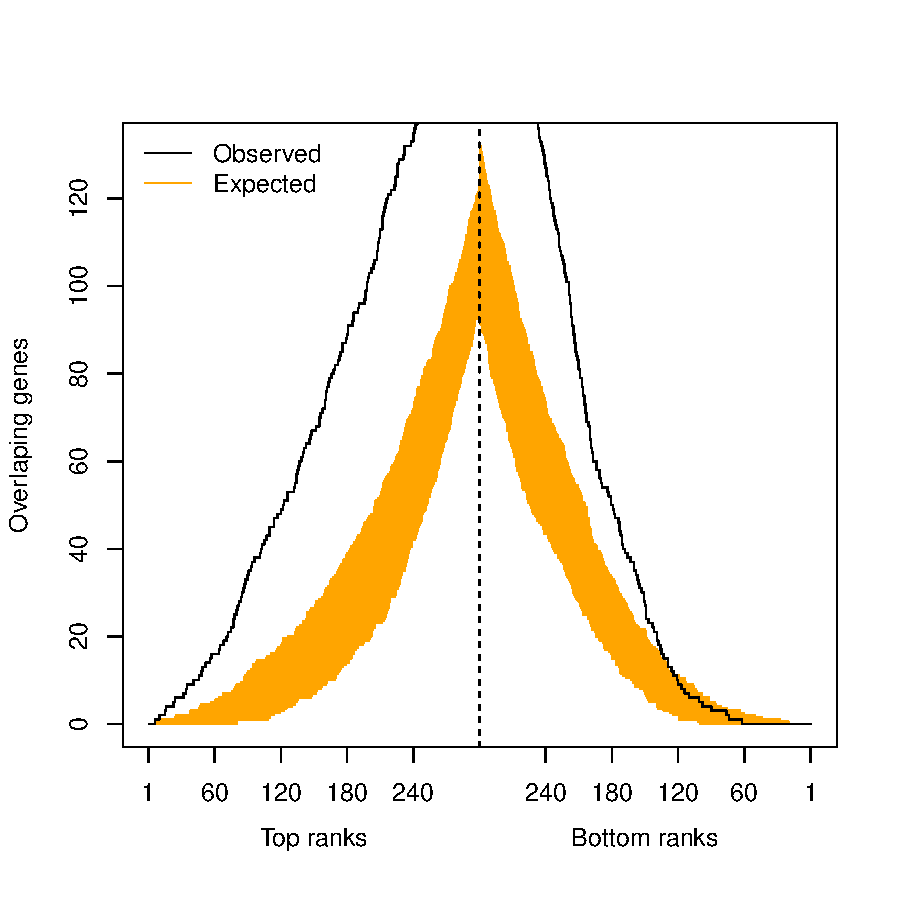
\includegraphics{MAMA-008}
    
The graph displays the empirical confidence intervals for number of overlapping genes to each position. Obsereved overlaps are drawn as black step-function.

\chapter{RankProduct}
%\addcontentsline{toc}{part}{RankProduct}
\section*{Introduction}
%\addcontentsline{toc}{section}{Introduction}
RankProduct is a non-parametric statistic that detects up-regulated and down-regulated genes under one condition against another condition. In our sample data set we look for difference in expression between MSI and MSS colon cancer. \par
It focuses on genes which are consistently highly ranked in a number of lists, for example genes that are regularly found among top up-regulated genes in many microarray studies. It assumes that under the null hypothesis the order of all items is random then the probability of finding a certain item among the top $r$ of $n$ items in a list is $p=r/n$. Rank product is defined by multiplying these probabilities $RP=\prod_{i}\frac{r_i}{n_i}$, where $r_i$ is the rank of the item in the $i$-th list and $n_i$ is the total number of the items on $i$-th list. The smaller the $RP$ value the smaller the probability that the observation of the item at the top of the lists is due to chance. It is equivalent to calculating the geometric mean rank. A list of up- or down-regulated genes are selected based on the estimated percentage of false positive prediction (pfp) - known as false discovery rate (FDR), too.
\section*{Algorithm}
Algorithm of the method has five steps:
\begin{enumerate}
\item Fold-change ratio is calculated in each data set.
\item Ranks are assigned (1 for the highest value) according to fold-change ratio. $r_{gi}$ is rank of gene $g$ in comparison $i$, where $i$ is from $1$ to $K$, where $K$ is sum of products of number of slides in groups.
\item RankProduct for a gene ($RP_g$) is calculated as $\prod_{i}r_{gi}^{1/K}$
\item $l$ permutations of expression values at each microarray slide is performed and all previous steps repeated. We obtain $RP_g^{(l)}$
\item Step 4 is repeated $L$ times to estimate the distribution of $RP_g^{(l)}$. This distribution is used to calculate p-value and pfp for each gene.
\end{enumerate}
\section*{Usage}
Function {\ttfamily RankProduct} provides the tables of identified up- and down- regulated genes from a MetaArray-class object.
\begin{Schunk}
\begin{Sinput}
> rp <- RankProduct(ColonData, "MSIstatus", num.perm = 50,
+  gene.names = rownames(GEDM(ColonData)[[1]]) )
\end{Sinput}
\begin{Soutput}
 The data is from  3 different origins 
 
Rank Product analysis for two-class case 
 
Starting  50 permutations... 
Computing pfp... 
Table1: Genes called significant under class1 < class2 

Table2: Genes called significant under class1 > class2 
\end{Soutput}
\end{Schunk}

\chapter{Z-statistic - posterior mean differential expression}
%\addcontentsline{toc}{part}{Z-statistic - posterior mean differential expression}
\section*{Introduction}
%\addcontentsline{toc}{section}{Introduction}
The main idea of this method is that one can use data from one study to construct a prior distribution of differential expression and thus utilize the posterior mean differential expression, weighted by variances, whose distribution is standard normal distribution due to classic Bayesian probability calculation. \par
It is based on assumption that gene expression is normally distributed with mean $\mu_g $ and SD $\sigma^2_g$ and that we can estimate $\sigma^2_g$ by pooling together all genes with similar levels of mean intensity. The difference in gene expression is tested by
\[ Z=\frac{D}{\sigma_D}=\frac{\overline{X}_1 - \overline{X}_2}{\sqrt{\frac{\sigma_1^2}{n_1}+\frac{\sigma_2^2}{n_2}}} \sim N(0,1),\]
where $\overline{X}_1$ and $\overline{X}_2$ denotes mean gene expression values in classes, $\sigma_1^2$ and $\sigma_2^2$ denotes the estimated SD in classes and $n_1$ and $n_2$ denotes the number of samples in classes. 
\section*{Usage}
Because the same number of samples in each class and study is used in primary publication of the method \cite{Wang}, we will first look at number of samples in our data.
\begin{Schunk}
\begin{Sinput}
> ColonData
\end{Sinput}
\begin{Soutput}
Dataset Denmark  containing 500 probes and  77 samples. 
Sumarization of samples: 
MSIstatus 
--------- 
MSI MSS 
 39  38 
age 
--- 
   Min. 1st Qu.  Median    Mean 3rd Qu.    Max. 
  36.00   45.00   54.00   54.92   62.00   80.00 

Dataset Australia  containing 500 probes and  36 samples. 
Sumarization of samples: 
MSIstatus 
--------- 
MSI MSS 
  5  31 
age 
--- 
   Min. 1st Qu.  Median    Mean 3rd Qu.    Max. 
  50.00   57.75   66.00   66.36   73.75   85.00 

Dataset Japan  containing 500 probes and  41 samples. 
Sumarization of samples: 
location 
-------- 
  distal proximal  unknown 
      28       11        2 
MSIstatus 
--------- 
MSI MSS 
 16  25 
age 
--- 
   Min. 1st Qu.  Median    Mean 3rd Qu.    Max. 
  40.00   47.00   53.00   53.61   60.00   65.00 
\end{Soutput}
\end{Schunk}
The smallest value in the tables above is 5, therefore we will randomly choose 5 samples in each class and data set. Function {\ttfamily posterior.mean} performs such data reduction and Z-statistic calculation. It has three required arguments: a data set as MetaArray object ({\ttfamily data}), name of clinical parameter with class labels ({\ttfamily  varname}) and number of samples to be selected ({\ttfamily nsamp}). 
\subsection*{Detecting differentially expressed genes}
We apply this method by
\begin{Schunk}
\begin{Sinput}
> z.stat<-posterior.mean(ColonData, "MSIstatus", nsamp=5)
\end{Sinput}
\begin{Soutput}
0 marked as 0
1 marked as 1
Contrast will be 1 - 0 
\end{Soutput}
\end{Schunk}
\subsection*{Results}
\begin{Schunk}
\begin{Sinput}
> head(round(z.stat,3))
\end{Sinput}
\begin{Soutput}
             Zscore Pvalue
1552281_at    4.179  0.000
1552365_at   -7.484  0.000
1552485_at   -2.410  0.016
1552502_s_at -0.300  0.764
1552546_a_at -0.418  0.676
1552553_a_at -0.057  0.955
\end{Soutput}
\end{Schunk}
Only values of Z-statistic ({\ttfamily Zscore}) and their p-values ({\ttfamily Pvalue}) are the outputs from this method.
\section*{Notes and discussion}
%\addcontentsline{toc}{section}{Notes and discussion}
This implementation expects either same microarray platform or same scale of expression values (like after POE transformation \cite{metaArray}) in all data sets.
         
          
\chapter{VennMapping}
%\addcontentsline{toc}{part}{VennMapping}
\section*{Introduction}
%\addcontentsline{toc}{section}{Introduction}
VennMapping \cite{Smid} is a method based on Venn diagrams and contingency tables. It looks for number of common genes in pairs of gene lists, statistical significance of observed match and returns also names of the common genes.
\section*{Algorithm}
%\addcontentsline{toc}{section}{Algorithm}
Algorithm of this method consists of three steps:
\begin{enumerate}
\item Calculation of fold-change in each data set.
\item Selection of significant (interesting) genes.
\item Comparison of gene lists pairs.
\end{enumerate}

\section*{Usage}
Function {\ttfamily VennMapper} selects genes in each dataset according to the fold-change cutoff and compares the lists of the selected genes.
\begin{Schunk}
\begin{Sinput}
> vm <- VennMapper(ColonData, varname="MSIstatus", cutoff=1)
> vm
\end{Sinput}
\begin{Soutput}
$conting.tab
          Denmark Australia Japan
Denmark        NA        12    16
Australia      12        NA     7
Japan          16         7    NA

$z.score
           Denmark Australia     Japan
Denmark         NA 14.964793 17.550323
Australia 14.93428        NA  8.098665
Japan     17.56230  8.120747        NA

$genes
          Denmark                                                                                                                                                                 
Denmark   NA                                                                                                                                                                      
Australia "205009_at;206239_s_at;37145_at;205044_at;213385_at;228030_at;205242_at;204818_at;206442_at;202917_s_at;202589_at;230793_at"                                            
Japan     "202803_s_at;230964_at;213915_at;206239_s_at;1556055_at;1552281_at;37145_at;209301_at;206391_at;230621_at;243669_s_at;228030_at;206442_at;209436_at;230793_at;228915_at"
          Australia                                                                                                                   
Denmark   "205009_at;206239_s_at;37145_at;205044_at;213385_at;228030_at;205242_at;204818_at;206442_at;202917_s_at;202589_at;230793_at"
Australia NA                                                                                                                          
Japan     "206239_s_at;209583_s_at;37145_at;228030_at;206442_at;210143_at;230793_at"                                                  
          Japan                                                                                                                                                                   
Denmark   "202803_s_at;230964_at;213915_at;206239_s_at;1556055_at;1552281_at;37145_at;209301_at;206391_at;230621_at;243669_s_at;228030_at;206442_at;209436_at;230793_at;228915_at"
Australia "206239_s_at;209583_s_at;37145_at;228030_at;206442_at;210143_at;230793_at"                                                                                              
Japan     NA                                                                                                                                                                      

attr(,"class")
[1] "VennMapper.res"
\end{Soutput}
\end{Schunk}
\emph{vm\$conting.tab} is the contingency table of the numbers of overlapping genes. \emph{vm\$z.score} is the table of z-scores corresponding to the overlaps and \emph{vm\$genes} is the table of the overlapping genes. 


\chapter{MAP-Matches}
%\addcontentsline{toc}{part}{MAP-Matches}
\section*{Introduction}
%\addcontentsline{toc}{section}{Introduction}
Meta-Analysis Pattern Matches (MAP-Matches) \cite{Yang2005} is a method that extends VennMapping \cite{Smid} and meta-profiling \cite{velkyRhodes}. It is designed to analyze more distinct microarray data (search for common molecular mechanism in all types of cancer). It assumes same gene set in all data sets. 
\section*{Algorithm}
%\addcontentsline{toc}{section}{Algorithm}
Algorithm of this method has five steps:
\begin{enumerate}
\item Calculation of T-statistic for each two classes in each data set. 
\item Building matrix of T-statistics (T-matrix) with rows referring to genes and columns to pairs of classes and data set.
\item Selection of threshold for T-statistic.
\item Transformation of T-matrix into a binary matrix: 1 for T-statistics above threshold, 0 for T-statistics below threshold.
\item Statistical analysis of transformed T-matrix (more details in Usage section).  
\end{enumerate}

\section*{Usage}
%\addcontentsline{toc}{section}{Usage}
Function {\ttfamily MAP.Matches} provides all steps of MAP-Matches method in one-line command. In
\begin{Schunk}
\begin{Sinput}
> map <- MAP.Matches(ColonData, "MSIstatus", t.cutoff = "95.00%", 
+ nperm = 100, sig.col = "p.col.strong")
\end{Sinput}
\begin{Soutput}
Examinig the data...
Statistical analysis...
Permutation: 
50 
100 
Permuting class labels in dataset: 
Denmark 
Australia 
Japan 
Permutation: 
50 
100 
\end{Soutput}
\end{Schunk}
the first argument is the dataset (MetaArray object), the second one is a column name of the class labels, {\ttfamily nperm} denotes the number of permutations and the last one {\ttfamily sig.col} is column name for selection of significant patterns - {\ttfamily "p.col.strong"} refer to the p-value of the strong matches when permutation of columns are used.

It returns a list of seven slots:
\begin{itemize}
\item \emph{tests} is a vector of test statistics
\item \emph{bin.matrix} is a matrix of genes selected in each of the datasets
\item \emph{sumarization} is a sumarization of \emph{bin.matrix}: the number of selected genes, the observed patterns and their empirical probabilities
\item \emph{MAP} is data frame with the numbers of observed strong or soft matches for each gene pattern
\item \emph{stat.analysis} extends \emph{summarization} with the p-values of the permutation-based tests of the statistical significance of the observed number of gene pattern matches
\item \emph{genes} is a list of gene names, where each slot refers to one gene pattern and contains the names of the genes for which the pattern was observed.
\item \emph{all.genes} is a vector of the names of the all genes in the analysis
\end{itemize}



\chapter{METRADISC}
%\addcontentsline{toc}{part}{METRADISC}
\section*{Introduction}
%\addcontentsline{toc}{section}{Introduction}
METRADISC \cite{Zintzaraz} is unique among rank-based methods because it provides an estimate of heterogeneity as one of its outputs. Additionally the method can deal with genes which are being measured in only some of the studies. The implementation available in MAMA package is restricted to genes common in all microarray studies analyzed.
\section*{Algorithm}
%\addcontentsline{toc}{section}{Algorithm}
\begin{enumerate}
\item Gene Ranking - In microarray analysis we usually test samples for a large number of genes. The results provide for each gene a test statistic and its statistical significance (p-value). Therefore we can rank the tested genes in each study based on direction in expression change and statistical significance. If there are $n$ genes being tested, the highest rank $n$ is given to the gene that shows the lowest $p$-value and it is up-regulated in diseased samples. Then follow all other up-regulated genes ranked according to increasing $p$-value. These are followed by down-regulated genes and the lowest rank ($1$) is given to gene that shows the lowest $p$-value and is down-regulated in diseased samples. Genes with equal $p$-values are assigned tied ranks. 
\item The Average Rank and Heterogeneity metrics - In this step we compute a average rank and heterogeneity metrics. The average rank $R^*$ is defined as $R^*= \frac{\sum_{i=1}^{s}R_i}{s}$, where $R_i$ is the rank of the gene in study $i$ and $s$ is total number of studies ($i=1,2,...,s$). The heterogeneity metrics $Q^*$ is given by formula $Q^*=\sum_{i=1}^{s}(R_i-R^*)^2$, it is actually generalization of Cochran's $Q$ statistic. 
\item Monte Carlo permutation test - To obtain statistical significance for average rank and heterogeneity metrics we randomly permute the ranks of each study and the stimulated metrics are calculated. Then we repeat the procedure to generate null distribution for the metrics. Each variable is then tested against the corresponding null distribution. We are interested genuinely in four statistical significances: for high average rank, for low average rank, for high heterogeneity and for low heterogeneity. Distinction between high and low average rank is important as we want to keep the direction of effect in mind. Ignoring it can lead to spurious results that a gene is consistently significant even if it is up-regulated in one study and down-regulated in second one. On the other hand, statistically low heterogeneity may suggest consistent results among different studies. The statistical significance for high average rank ($R^*$) is defined as the percentage of simulated metrics that exceed or are equal to the observed ($R^*$). The statistical significance for low average rank ($R^*$) is defined as the percentage of simulated metrics that are below or equal to the observed ($R^*$). Significance of heterogeneity is defined analogously.  
\end{enumerate}
\section*{Usage}
%\addcontentsline{toc}{section}{Usage}
Function {\ttfamily METRADISC} performs all steps of this method in one command.
\begin{Schunk}
\begin{Sinput}
> metra<-METRADISC(ColonData, "MSIstatus", nperm = 1000)
\end{Sinput}
\begin{Soutput}
100   200   300   400   500   600   700   800   900   1000   
\end{Soutput}
\begin{Sinput}
> str(metra)
\end{Sinput}
\begin{Soutput}
List of 3
 $ ranks :'data.frame':	500 obs. of  3 variables:
  ..$ Denmark  : num [1:500] 105 326 348 390 473 484 83 126 498 482 ...
  ..$ Australia: num [1:500] 368 257 488 397 170 424 179 187 490 495 ...
  ..$ Japan    : num [1:500] 156 153 380 442 445 419 88 187 390 469 ...
 $ RQ    : num [1:500, 1:2] 210 245 405 410 363 ...
  ..- attr(*, "dimnames")=List of 2
  .. ..$ : chr [1:500] "217562_at" "203766_s_at" "1554394_at" "212662_at" ...
  .. ..$ : chr [1:2] "r.star" "q.star"
 $ MCtest: num [1:500, 1:4] 0.659 0.548 0.021 0.027 0.098 0.009 0.957 0.832 0 0 ...
  ..- attr(*, "dimnames")=List of 2
  .. ..$ : chr [1:500] "217562_at" "203766_s_at" "1554394_at" "212662_at" ...
  .. ..$ : chr [1:4] "R.high" "R.low" "Q.high" "Q.low"
 - attr(*, "class")= chr "METRADISC.res"
\end{Soutput}
\end{Schunk}
It returns a list with ranks for each gene and dataset {\emph ranks}, average rank and heterogeneity for each gene {\emph RQ} and results of the Monte Carlo test {\emph MCtest}.


\chapter{Results combination}
%\section{Methods comparison}
In this chapter we are going to compare and combine outputs from all methods so we can look and changes in gene expression in various ways. \par
We are going to start with lists of differentially expressed genes, because this is the only one output common for all methods mentioned in this vignette. We will merge all lists into one variable via function {\ttfamily join.DEG}.
\begin{Schunk}
\begin{Sinput}
> lists<-join.DEG(pval, es, es2, SOGL.res, rp, z.stat,
+   map,  cutoff=0.05)
> names(lists)<-c("PvalCom", "ESCom","ESCom2","OrderedList",
+ "RankProduct", "Z-stat","MAP")
> summary(lists)
\end{Sinput}
\begin{Soutput}
            Length Class  Mode     
PvalCom     212    -none- character
ESCom       166    -none- character
ESCom2      195    -none- character
OrderedList 104    -none- character
RankProduct 176    -none- character
Z-stat      169    -none- character
MAP          18    -none- character
\end{Soutput}
\end{Schunk}
Now, we will transform this list to a binary matrix where rows refer to genes and columns to method and $1$ means that the gene was identified as a differentially expressed gene in the method. Function {\ttfamily make.matrix} provides such transformation.  
\begin{Schunk}
\begin{Sinput}
> MAT<-make.matrix(lists)
> MAT[1:5,1:5]
\end{Sinput}
\begin{Soutput}
             PvalCom ESCom ESCom2 OrderedList RankProduct
1554394_at         1     0      1           0           0
212662_at          1     1      1           0           0
1555370_a_at       1     0      0           0           1
240574_at          1     1      1           0           1
203553_s_at        1     1      1           0           0
\end{Soutput}
\end{Schunk}
It is very popular to visualize results of microarray analysis as a heatmap. A heatmap is a graphical representation for a numeric matrix where values are presented as colors. Gene expression values are usually used in microarray analysis. In these pictures colors go continuously from green (for down-regulation) through black (for no change in gene expression) to red (for up-regulation). There are several R-packages which implement plotting heatmaps in slightly different way. Functions {\ttfamily metaheat} and {\ttfamily metaheat2} are modification of two of them, so a discrete set of colors (only two in {\ttfamily metaheat} but even several in {\ttfamily metaheat2}) can be used with an appropriate legend.\par
Function {\ttfamily metaheat} has three arguments: a data matrix ({\ttfamily MAT}), a number defining position of legend ({\ttfamily legend=1} is legend drawn below the picture) and vector of colors ({\ttfamily col}). 
\begin{center}
\begin{Schunk}
\begin{Sinput}
> metaheat(MAT, legend=1, col=c("red3", "royalblue2"))
\end{Sinput}
\end{Schunk}
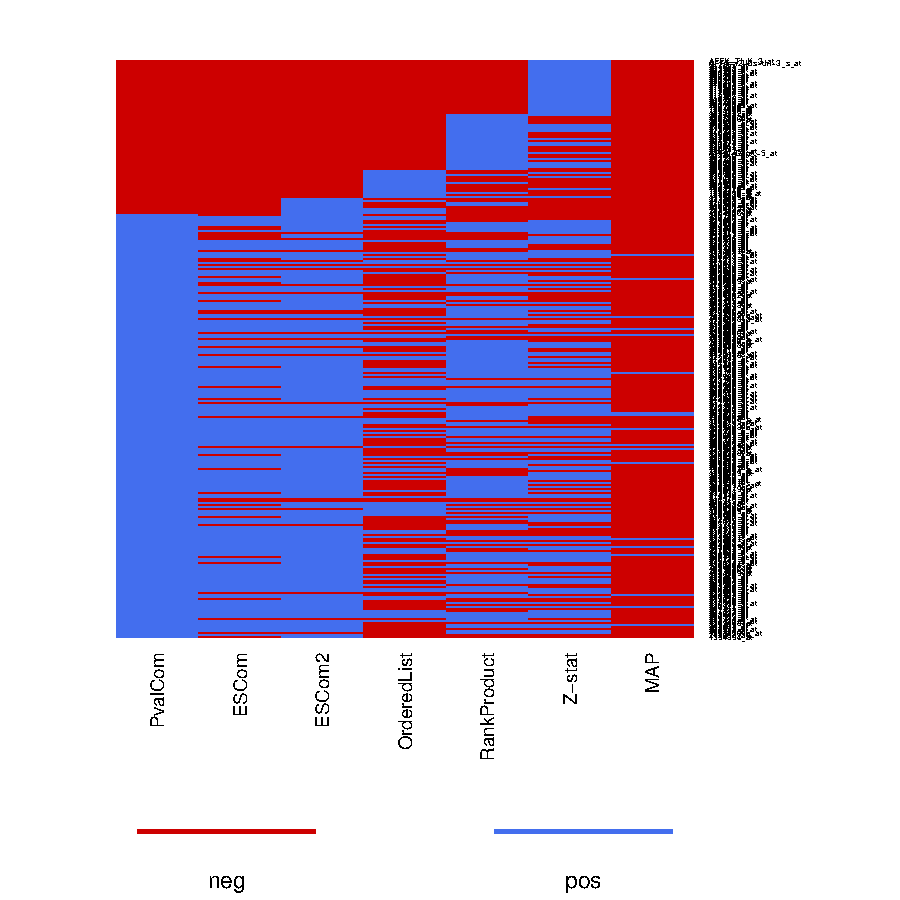
\includegraphics{MAMA-018}
\end{center}                  
 Function {\ttfamily metaheat2} has as many arguments as {\ttfamily heatmap.2} form gplots package and two more. Argument {\ttfamily legend.names} is a character vector with labels to be used in legend. Setting {\ttfamily discret=TRUE} will indicate that legend for discrete values should be drawn. 
\begin{center}
\begin{Schunk}
\begin{Sinput}
> metaheat2(MAT, col=c("red3", "royalblue2"), legend.names=c("DEG",
+ "noDEG"), discrete=TRUE, trace="none", 
+ dendrogram="none", cexCol=0.9)
\end{Sinput}
\end{Schunk}
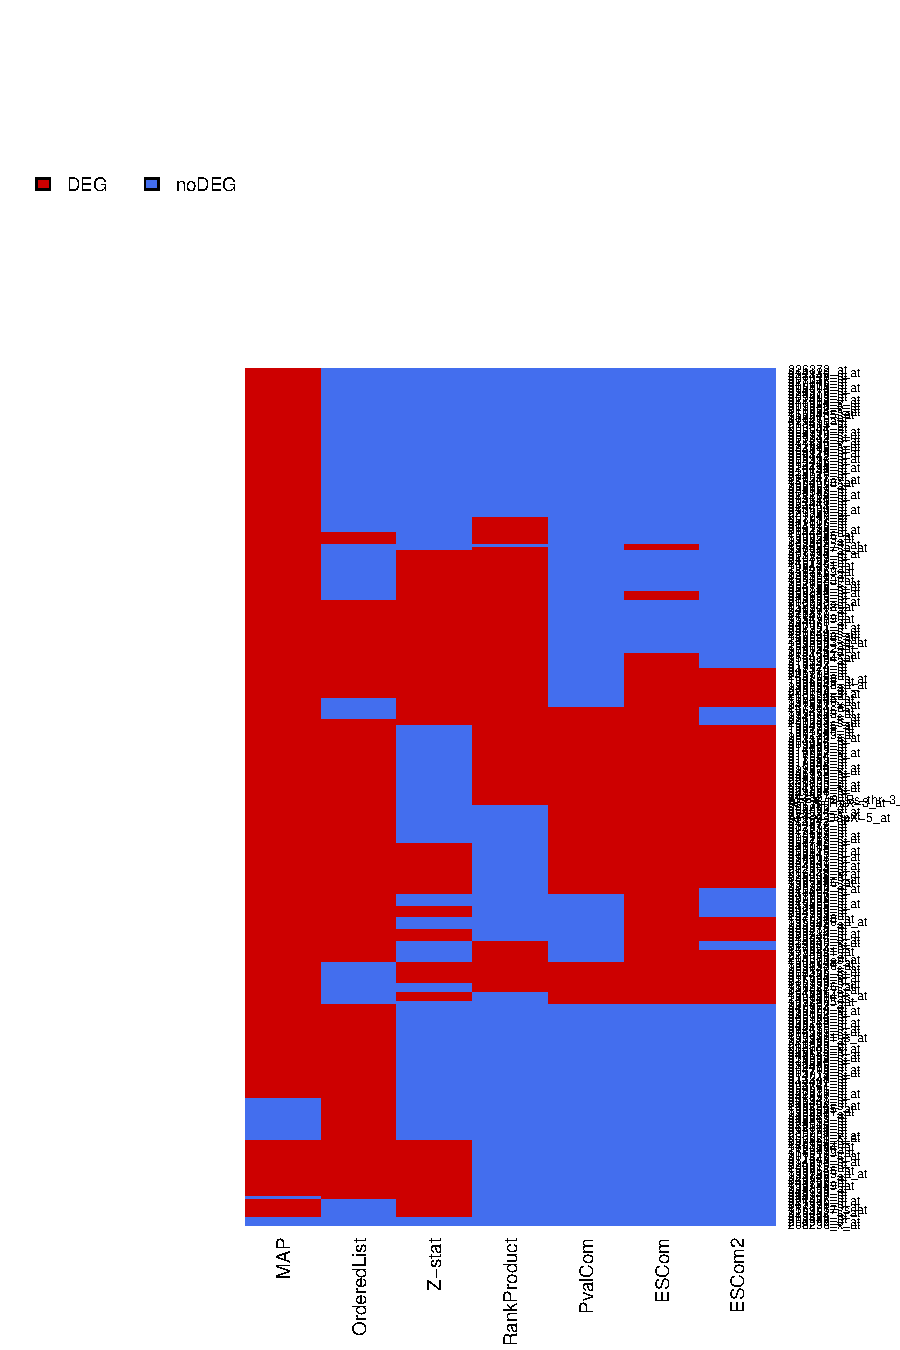
\includegraphics{MAMA-019}
\end{center}
The user can perform cluster analysis on {\ttfamily MAT} to search for similarities between methods or genes.\par
We can look at number of genes found by number of methods by
\begin{Schunk}
\begin{Sinput}
> dim(MAT)
\end{Sinput}
\begin{Soutput}
[1] 289   7
\end{Soutput}
\end{Schunk}
According to the outsprint above, eight different methods have found more than 270 differentially expressed genes. \par
The histogram below shows that the most of the genes have been selected in only one method. 
\begin{center}
\begin{Schunk}
\begin{Sinput}
> n.met<-apply(MAT,1,sum)
> hist(n.met, main="", xlab="Number of methods", 
+ ylab="Number of genes", xlim=c(1,8))
\end{Sinput}
\end{Schunk}
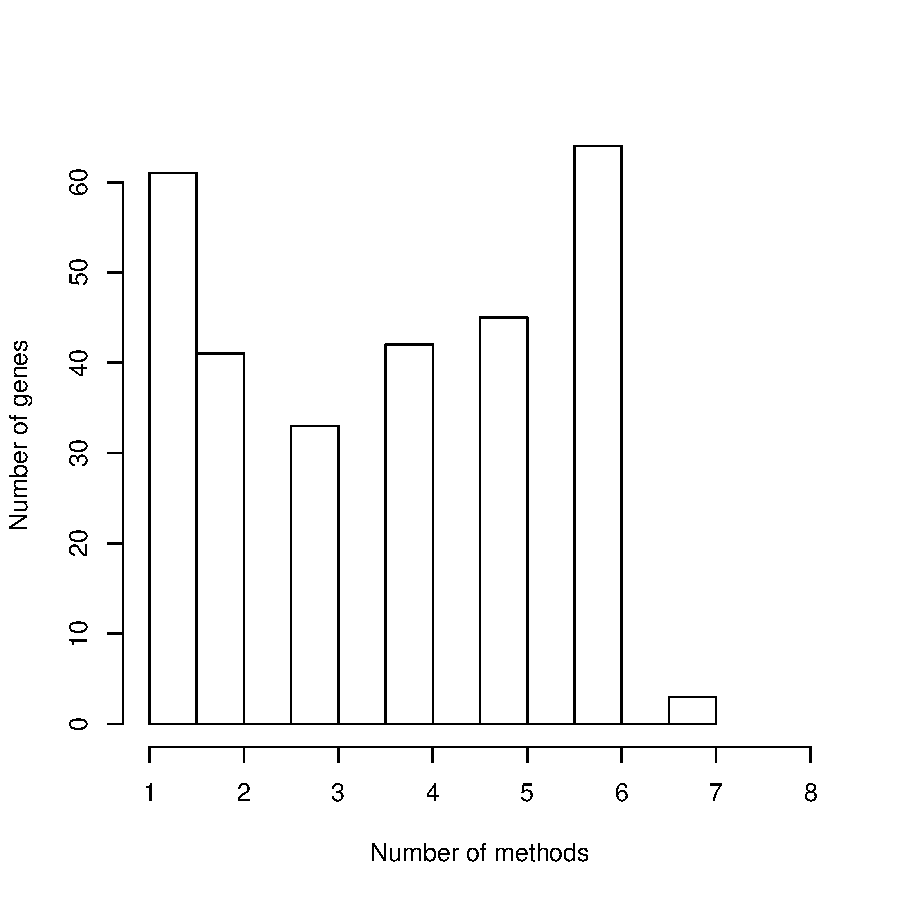
\includegraphics{MAMA-021}
\end{center}
{\ttfamily n.met} is a numeric vector of number of methods that identified the gene as differentially expressed. \par 
Next, we can look for example how many genes have been found as differentially expressed in at least 6 methods.
\begin{Schunk}
\begin{Sinput}
> dim(MAT[n.met>5,])
\end{Sinput}
\begin{Soutput}
[1] 67  7
\end{Soutput}
\end{Schunk}
On the other hand, we can find out how many genes have been found by a method.
\begin{center}
\begin{Schunk}
\begin{Sinput}
> n.gen<-apply(MAT,2,sum)
> barplot(n.gen, cex.names=0.8, las=2)
\end{Sinput}
\end{Schunk}
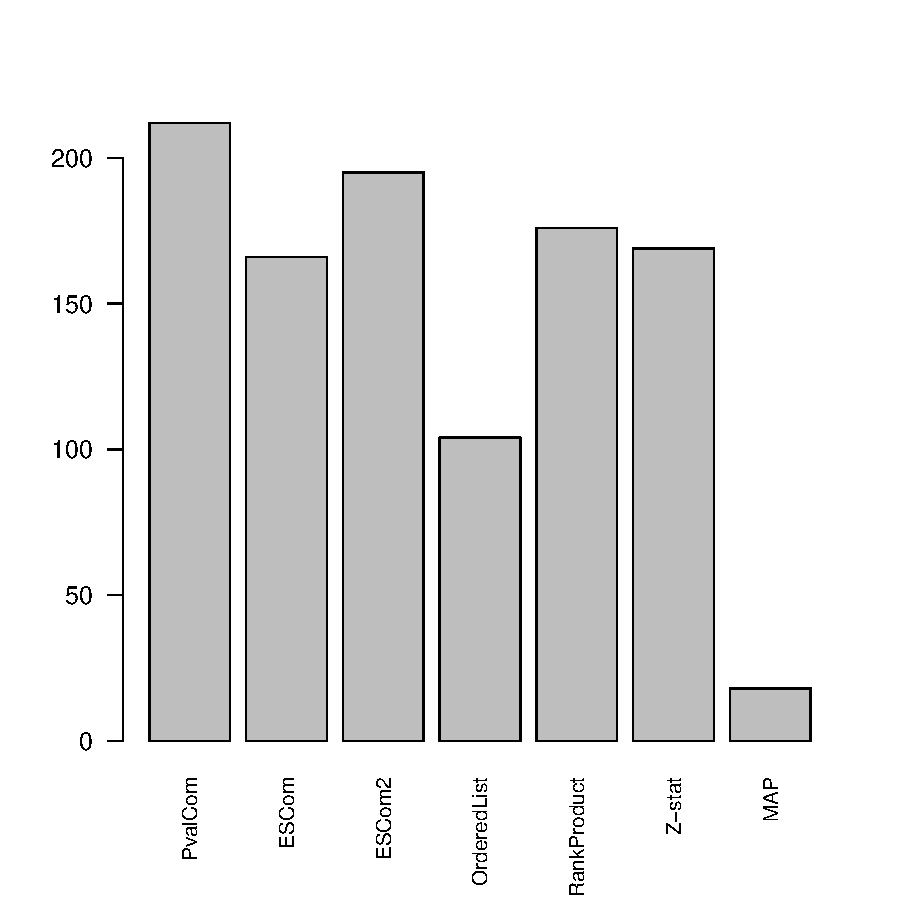
\includegraphics{MAMA-023}
\end{center}
Function {\ttfamily contig.tab} provides a number of genes common in two gene lists. It can be applied to {\ttfamily lists}, too.
\begin{Schunk}
\begin{Sinput}
> TAB<-conting.tab(lists)
> TAB[1:5,1:5]
\end{Sinput}
\begin{Soutput}
            PvalCom ESCom ESCom2 OrderedList RankProduct
PvalCom          NA   166    187          86         142
ESCom           166    NA    166          78         125
ESCom2          187   166     NA          87         136
OrderedList      86    78     87          NA          64
RankProduct     142   125    136          64          NA
\end{Soutput}
\end{Schunk}
%Integration Driven Discovery (IDD) and Integration Driven Revision (IDR) became popular for methods which combine p-values or effect sizes. IDD is a gene that has been found significant in meta-analysis but not in any of one data set analyses. A gene that is significant only in one data set analysis and not in meta-analysis is called IDR. A high number of IDD suggests that the method is capable to catch small but constant changes in gene expression, whereas high number of IDR is being explained as capability to suppress great expression changes observed in only one data set.\par % Function {\ttfamily makeIDDIDRtable()} provides IDD/IDR characteristic of all 

\section*{Expression of one gene}
In this section we are going to focus on one gene and to look at its expression change from different points of view. The different points of view are represented by different approaches used in the methods.\par
First we will join all the available results to one list and then select only rows for one gene.\par

\begin{Schunk}
\begin{Sinput}
> results<-join.results(pval, es, es2, SOGL.res, rp, z.stat, map, metra)
> gene<-metagene("203008_x_at",results)
> names(gene)<-c("pval","es.metaMA", "es.GeneMeta", "SOGL", "RP",
+  "z.stat", "MAP", "METRADISC")
> gene
\end{Sinput}
\begin{Soutput}
$pval
       study1        study2        study3 AllIndStudies 
     1.000000      1.000000      1.000000      1.000000 
         Meta TestStatistic 
     1.000000      8.732214 
attr(,"class")
[1] "metaMA"      "metaMA.gene"

$es.metaMA
       study1        study2        study3 AllIndStudies 
     1.000000      1.000000      1.000000      1.000000 
         Meta TestStatistic 
     1.000000     -8.492688 
attr(,"class")
[1] "metaMA"      "metaMA.gene"

$es.GeneMeta
     zSco_Ex_1      zSco_Ex_2      zSco_Ex_3           zSco 
   -6.44329249    -3.76525489    -4.69659562    -8.80275939 
        MUvals          MUsds          Qvals             df 
   -1.77309287     0.20142467     0.26260012     2.00000000 
      Qpvalues          Chisq    Effect_Ex_1    Effect_Ex_2 
    0.87695460     0.00000000    -1.71847860    -2.02486588 
   Effect_Ex_3 EffectVar_Ex_1 EffectVar_Ex_2 EffectVar_Ex_3 
   -1.75867849     0.07113324     0.28920365     0.14021890 
     zSco_Ex_1       FDR_Ex_1      zSco_Ex_2       FDR_Ex_2 
   -6.44329249     0.00000000    -3.76525489     0.02125000 
     zSco_Ex_3       FDR_Ex_3           zSco            FDR 
   -4.69659562     0.00000000    -8.80275939     0.00000000 
        MUvals          MUsds          Qvals             df 
   -1.77309287     0.20142467     0.26260012     2.00000000 
      Qpvalues          Chisq 
    0.87695460     0.00000000 
attr(,"class")
[1] "ES.GeneMeta"      "ES.GeneMeta.gene"

$SOGL
NULL
<0 rows> (or 0-length row.names)

$RP
        gene.index            RP/Rsum FC:(class1/class2) 
          415.0000            78.6607             0.5803 
               pfp            P.value 
            0.0000             0.0000 
attr(,"class")
[1] "RankProduct"      "RankProduct.gene"

$z.stat
              Zscore       Pvalue
203008_x_at 4.342487 1.408791e-05

$MAP
 110  101  011  111 
TRUE TRUE TRUE TRUE 
attr(,"class")
[1] "MAP.Matches"      "MAP.Matches.gene"

$METRADISC
r.star q.star R.high  R.low Q.high  Q.low 
   497     38      0      1      1      0 
attr(,"class")
[1] "METRADISC"      "METRADISC.gene"

attr(,"class")
[1] "metagene"
\end{Soutput}
\end{Schunk}
This output provides much of the information available on the gene through all the described methods. It is a rather complicated structure, so we will try to represent it graphically in comprehensible form.
\begin{center}
\begin{Schunk}
\begin{Sinput}
> plotgene(gene, datalabels=c("denmark", "australia", "japan", "combined"))
\end{Sinput}
\end{Schunk}
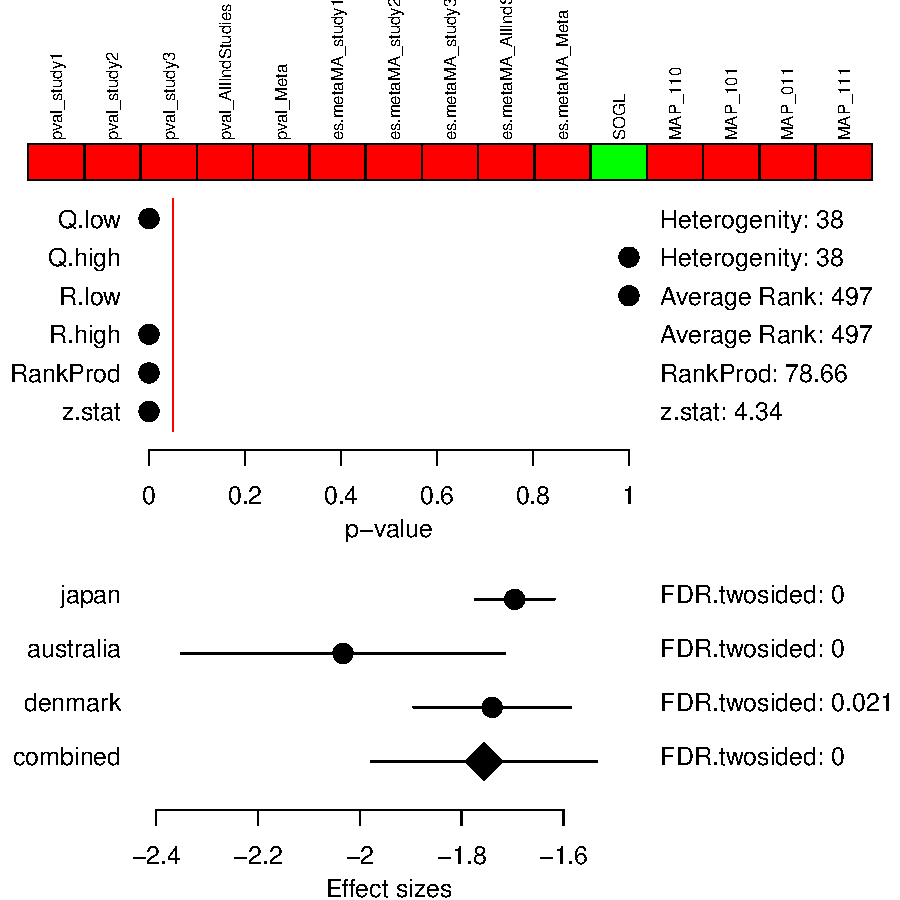
\includegraphics{MAMA-026}
\end{center}
The picture above shows in top part occurrence of gene in lists of selected genes in some methods.  The dark box means that the gene is present in the list. Values from objects: {\ttfamily pvalt}, {\ttfamily ESt}, {\ttfamily x.z} and {\ttfamily probs} are used in here. \par
The middle part is dedicated to p-values available in meta-analysis. Specific values of the statistics can be found on the right side of the chart. The vertical dashed line denotes the signifficance threshold $5\%$. P-values from {\ttfamily MC}, {\ttfamily RankRes} and {\ttfamily z.stat} are drawn in here.\par
Combination of effect size is plotted in the bottom graph. The point marks the effect size. Horizontal lines denote the variance of effect size. Statistical significance of the difference in gene expression (FDR adjusted) can be found on the right side of the chart. This graph uses values from {\ttfamily theScores} and {\ttfamily ScoresFDR}.

\begin{thebibliography}{99}
\bibitem{ausaden}Jorissen, R. N., Lipton, L., Gibbs, P., Chapman, M. et al. 2008, \emph{DNA copy-number alterations underlie gene expression differences between microsatellite stable and unstable colorectal cancers}, Clinical Cancer Research, Vol. 14, pp. 8061-8069
\bibitem{japan}Watanabe, T., Kobunai, T., Toda, E., Yamamoto, Y. et al. 2006, \emph{Distal colorectal cancers with microsatellite instability (MSI) display distinct gene expression profiles that are different from proximal MSI cancers} Cancer Research, Vol.66, no. 20, pp. 9804-9808
\bibitem{Biobase}Falcon, S., Morgan, M. and Gentleman, R. 2007, \emph{An introduction to Biocinductor's ExpressionSet class}, available at: http://www.bioconductor.org/packages/2.2/bioc/vignettes/Biobase/inst /doc/ExpressionSetIntroduction.pdf
\bibitem{Marot}Marot, G., Foulley, J.L., Mayer, C.D.,Jaffrezic, F. 2009, \emph{Moderated effect size and P-value combinations for microarray meta-analyses}, Bioinformatrics, Vol. 25 no. 20 2009, pp. 2692-2699
\bibitem{Rhodes}Rhodes, D.R., Barrette, T.R., Rubin, M. A., Ghosh, D. a Chinnaiyan, A. M. 2002, \emph{Meta-Analysis of Microarrays: Interstudy Validation of Gene Expression Profiles Reveals Pathway Dysregulation in Prostate Cancer}, CANCER RESEARCH 62, pp: 4427-4433
\bibitem{Fisher25}Fisher, R.A. 1925, \emph{Statistical methods for research}, Oliver and Boyd, Edinburgh
\bibitem{limma}Smyth, G. K. 2004, \emph{Linear models and empirical Bayes methods for assessing differential expression in microarray experiments}, Statistical Applications in Genetics and Molecular Biology 3, No. 1, Article 3
\bibitem{SMVar}Jaffrezic, F., Marot, G., Degrelle, S., Hue, I., Foulley, J.L. 2007, \emph{A structural mixed model for variances in differential gene expression studies}, Genetical Research, Vol. 89, pp. 19-25.
\bibitem{Choi2003}Choi, J.K., Yu, U., Kim, S. a Yoo, O.J. 2003, \emph{Combining multiple microarray studies and modeling interstudy variation}, Bioinformatics, Vol. 19, Suppl. 1 2003, pp. i84-i90
\bibitem{GeneMeta}Gentleman, R., Rauschhaupt, M., Huber, W., a Lusa L. 2008, \emph{Meta-analysis for Microarray Experiments}, available at: http://www.bioconductor.org/packages/2.3/bioc/vignettes/GeneMeta /inst/doc/GeneMeta.pdf 
\bibitem{Hedges}Hedged, V. L. a Olkin, I. 1985, \emph{Statistical Methods for Metaanalysis}, Academic Press, Orlando
\bibitem{Cochran}Cochran, B.G. 1954, \emph{The combination of estimates from different experiments}, Biometrics, Vol. 10, pp. 101-129
\bibitem{DerSimonian}DerSimonian, R., a Laird, N. M. 1986, \emph{Meta-analysis in clinical trials}, Controlled Clinical Trials, Vol. 7, pp. 177-188
\bibitem{SOGL}Scheid, S., Lottaz, C., Yang, X. a Spang, R. 2006, \emph{Similarities of Ordered Gene Lists User's Guide to the Bioconductor Package OrderedList 1.11.3}, availale at: http://www.bioconductor.org/packages/2.5/bioc/vignettes/
OrderedList/inst/doc/tr\_2006\_01.pdf
\bibitem{Hong}Hong, F., Breitling, R., McEntee,C. W., Wittner, B. S., Nemhauser, J. L. a Chory, J. 2006, \emph{RankProd: a bioconductor package for detecting differentially expressed genes in meta-analysis}, Bioinformatics, Vol. 22, no. 22 2006, pp. 2825-2827
\bibitem{Wang}Wang, J., Coombes, K. R., Highsmith, W. E., Keating, M. J. a  Abruzzo, L. V. 2004, \emph{Differences in gene expression between B-cell chronic lymphocytic leukemia and normal B cells: a meta-analysis of three microarray studies}, Bioinformatics, Vol. 20, no. 17 2004, pp. 3166-3178
\bibitem{metaArray} Ghosh, D. a Choi, H. 2009, \emph{metaArray package for meta-analysis of microarray data}, available at: http://bioconductor.org/packages/2.5/bioc/vignettes/metaArray/inst/ doc/metaArray.pdf
\bibitem{Geman}Geman, D., d'Avignon, Ch., Naiman, D. Q. a Winslow, R.L. 2004, \emph{Classifying Gene Expression Profiles from Pairwise mRNA Comparisons}, Statistical Applications in Genetics and Molecular Biology 2004, Vol. 3, Issue 1, Article 19
\bibitem{Tan} A.C. Tan, D.Q. Naiman, L. Xu, R.L. Winslow, D. Geman, \emph{Simple decision rules for classifying human cancers from gene expression profiles}, Bioinformatics, 21: 3896-3904, 2005.
\bibitem{Smid}Smid, M., Dorssers, L. C. J. a Jenster, G. 2003, \emph{Venn Mapping: clustering of heterologous microarray data based on the number of co-occurring differentially expressed genes}, Bioinformatics, Vol. 19, no. 16 2003, pp. 2065-2071
\bibitem{Yang2005}Yang, X., Bentink, S. a Spang, R. 2005, \emph{Detecting Common Gene Expression Patterns in Multiple Cancer Outcome Entities}, Biomedical Microdevices, Vol.7:3, pp. 247-251
\bibitem{velkyRhodes}Rhodes, D. R., Yu, J., Shanker, K., Deshpande, N., Varambally, R., Ghosh, D., Barrette, T., Pandey, A. a Chinnaiyan, A. M. 2004, \emph{Large-scale meta-analysis of cancer microarray data identifies common transcriptional profiles of neoplastic transformation and progression}, PNAS, Vol. 101, no. 25, pp. 9309-9314
\bibitem{Zintzaraz}Zintzaraz, E a Ioannidis, J.P.A. 2008, \emph{Meta-analysis for ranked discovery datasets: Theoretical framework and empirical demonstration for microarrays}, Computational Biology and Chemistry 32, pp. 39-47
%\bibitem{Heatplus}
%\bibitem{gplots}
\end{thebibliography}
\end{document}

